% !TeX program = xelatex
\RequirePackage[OT1]{fontenc}
\documentclass[letterpaper,10pt,journal]{IEEEtran}
\usepackage{fontspec}
\setmainfont{TeX Gyre Termes}
\setsansfont{TeX Gyre Heros}
\setmonofont{TeX Gyre Cursor}
\usepackage{amsmath,amssymb,bm,graphicx,booktabs,tabularx,array,url,cite}
\graphicspath{{figures/}}
\interdisplaylinepenalty=2500
\newenvironment{practitioners}{\renewcommand{\abstractname}{Note to Practitioners}\begin{abstract}}{\end{abstract}}
\newcommand{\pose}{\bm{q}}
\newcommand{\NA}{N/A}
\title{LogicFly: Conditional Task Graphs and Joint Task--Viewpoint Planning for Language-Guided Aerial Navigation}
\author{Anonymous Author(s)}
\markboth{IEEE Transactions on Automation Science and Engineering}{Anonymous Author(s): LogicFly}
\begin{document}
\maketitle
\begin{abstract}
Robots assisting with household tasks must interpret long, natural-language instructions that resemble everyday human requests and coordinate multiple subtasks linked by complex logical constraints. Such instructions combine spatial references, mandatory precedence, freely ordered subtasks, and observation-dependent conditional branches, requiring joint decisions about what to do next and where to obtain visual evidence. We present \textbf{LogicFly}, a language-guided framework for household navigation, search, and visual verification, implemented on an aerial robot using a reusable 3D semantic map constructed through fully autonomous exploration. A Conditional Partial-Order Task Graph (CPTG) represents long-horizon instructions by separating task dependencies from observation-triggered branch rules. Joint Task--Viewpoint Planning (JTVP) jointly selects task order and observation poses within a rolling task window, accounting for collision-checked 3D paths, motion time, visibility, and terminal observation costs. Online RGB-D verification updates task states and triggers bounded semantic-region search when a mapped location is unproductive. Under full-task scoring on a project-authored benchmark of six HM3D scenes, LogicFly achieves success rates of 93.33\% on single-target tasks and 71.11\% on multi-target tasks. We further validate the framework on a physical UAV, demonstrating real-world execution of complex multi-target tasks with logical dependencies among subtasks.
\end{abstract}

% T-ASE requires a 100--300 word practitioner-oriented note after the abstract.
\begin{practitioners}
This work is motivated by indoor service tasks in which a robot must inspect several locations, respect a required order, and decide what to do next from what it observes. Examples include household item checks and repeated visual inspection in buildings. The proposed system first builds a reusable three-dimensional map, then converts a request into tasks with explicit dependencies. It chooses both the visit order and the camera positions, and revises the remaining plan when an expected object is missing. This can reduce unnecessary travel while preserving the conditions attached to each task. Deployment requires a mapped environment, reliable localization, a depth camera, and collision-aware motion control. The reported simulation benchmark uses precompiled task graphs, so its results do not establish the reliability of interpreting arbitrary user requests. Physical flights demonstrate feasibility, but broader operational reliability has not been established. Object recognition errors, incomplete maps, and changing environments remain practical limitations. Further validation is needed before extending the approach to routine inventory checks or inspection services in occupied buildings.
\end{practitioners}

\begin{IEEEkeywords}
Aerial robotics, task and motion planning, vision-and-language navigation, semantic mapping, visual verification.
\end{IEEEkeywords}

\begin{figure*}[t]
\centering
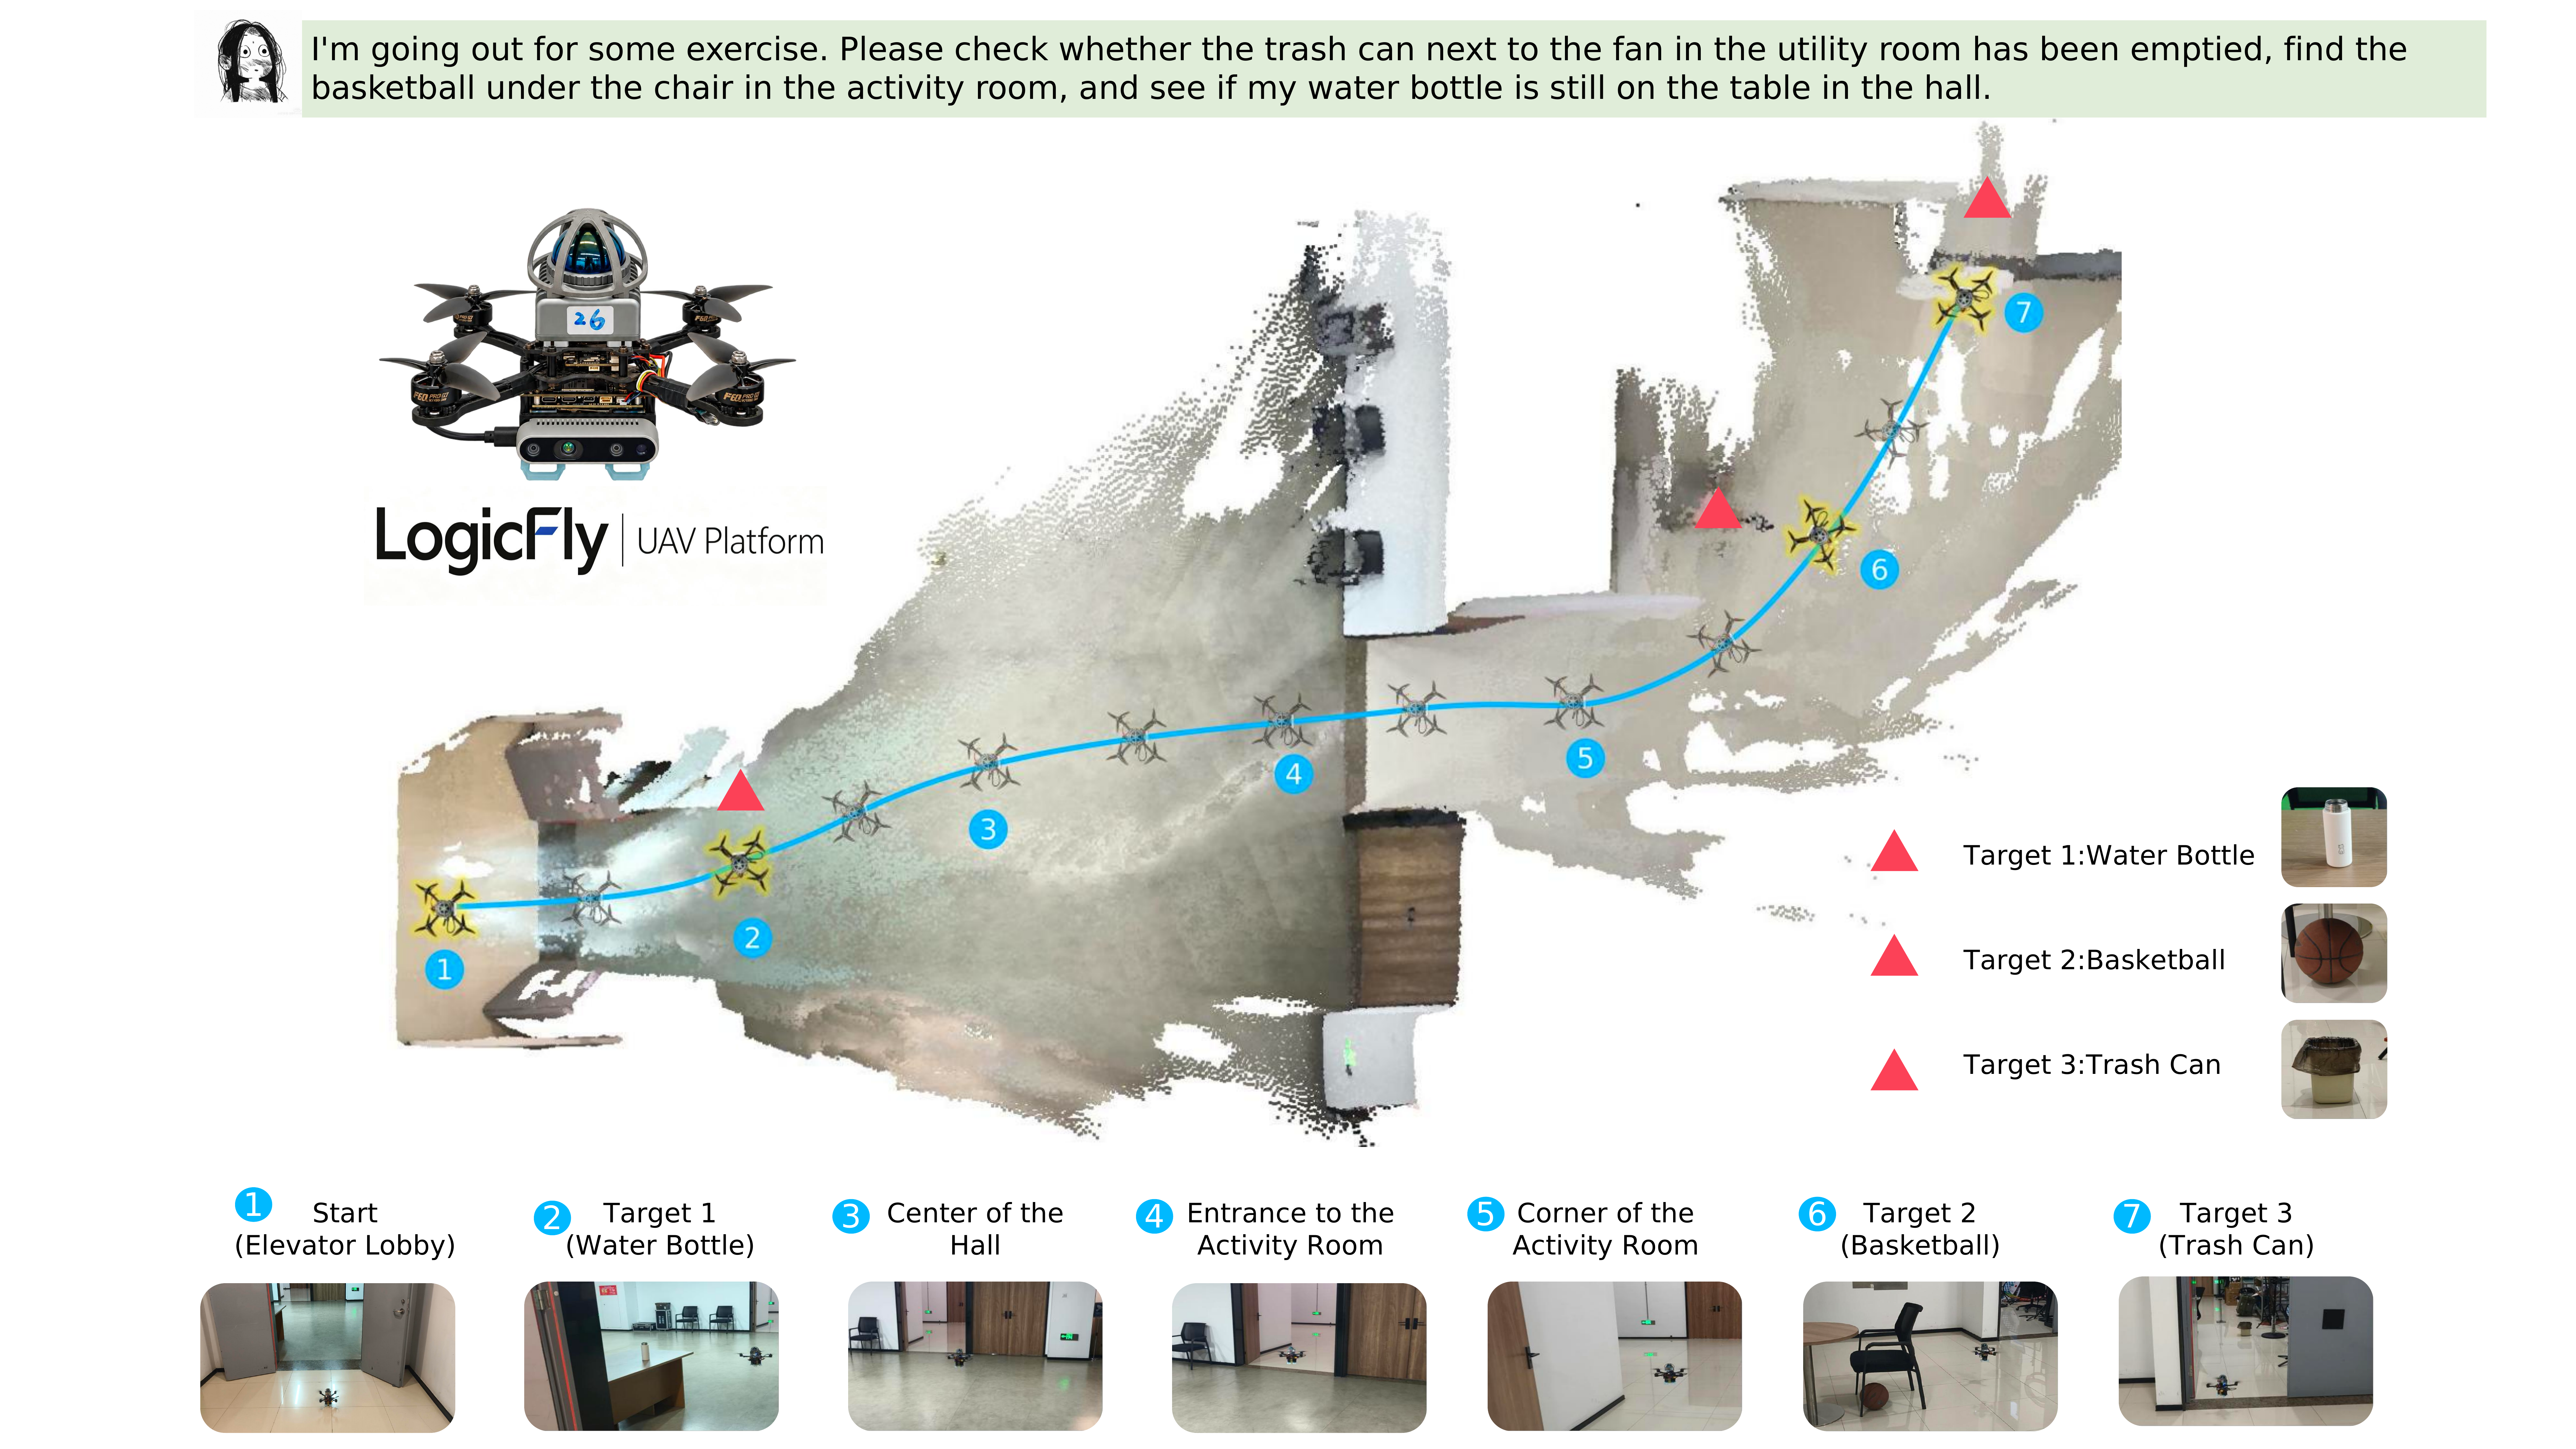
\includegraphics[width=\textwidth]{real_world_execution.png}
\caption{Real-world execution of LogicFly. A physical UAV completes a three-target task in a real multi-room environment. Because the complete environment cannot be captured in a single overhead photograph, its 3D reconstruction is used only to visualize the physical layout and the executed trajectory. Numbered camera views show the real flight sequence from takeoff to task completion.}
\label{fig:real-world-main}
\end{figure*}


\section{Introduction}
Vision-and-Language Navigation (VLN) connects natural-language instructions with embodied robot motion in visually observed environments. Representative benchmarks such as R2R~\cite{anderson2018r2r} and VLN-CE~\cite{krantz2020vlnce} have driven substantial progress in instruction following and continuous-space navigation, while ALFRED~\cite{shridhar2020alfred} further highlights the difficulty of grounding long, compositional household directives into state-dependent action sequences. However, most conventional VLN formulations focus on relatively compact navigation goals or sequential route-following instructions, without explicitly modeling the complex task logic that arises when multiple interdependent subtasks must be executed within a single instruction.

Real-world language-guided tasks often involve precedence constraints, flexible execution orders, spatial relations, and observation-dependent decisions rather than a single destination or fixed route. The robot must determine not only which task to execute next, but also where to obtain reliable visual evidence and how geometric travel costs should influence task ordering. Moreover, newly acquired observations may alter the current task state, redirect subsequent search, or activate or skip downstream tasks. For example, an instruction may require checking one object first, searching for another under a spatial constraint, and activating additional search only when the expected target is absent. These coupled requirements motivate a unified closed-loop framework that jointly reasons over task logic, observation geometry, and motion planning.

This setting changes both the planning objective and the meaning of success. Reaching every mentioned object is insufficient if the robot violates a required precedence relation, visits a branch that should have been skipped, or observes the correct category from a pose that cannot establish the requested relation. Conversely, an efficient executor should retain freedom among unordered subtasks and exploit that freedom to reduce geometric travel. The task representation must therefore preserve logical constraints without unnecessarily imposing a single language order, and execution must couple those constraints to observable geometric goals.

To support such execution in initially unknown environments, the system first constructs a reusable hierarchical semantic--geometric representation through autonomous aerial exploration. The representation jointly organizes occupied and free space, floors, rooms, cross-floor transitions, and open-vocabulary object instances, providing both the geometric structure required for navigation and the semantic grounding needed for subsequent language-conditioned tasks. Our central focus is how to exploit this autonomously constructed representation to execute language instructions involving complex logical dependencies and spatial constraints through structured task reasoning, task-conditioned 3D observation poses, and collision-aware motion planning.

\begin{figure*}[t]
\centering
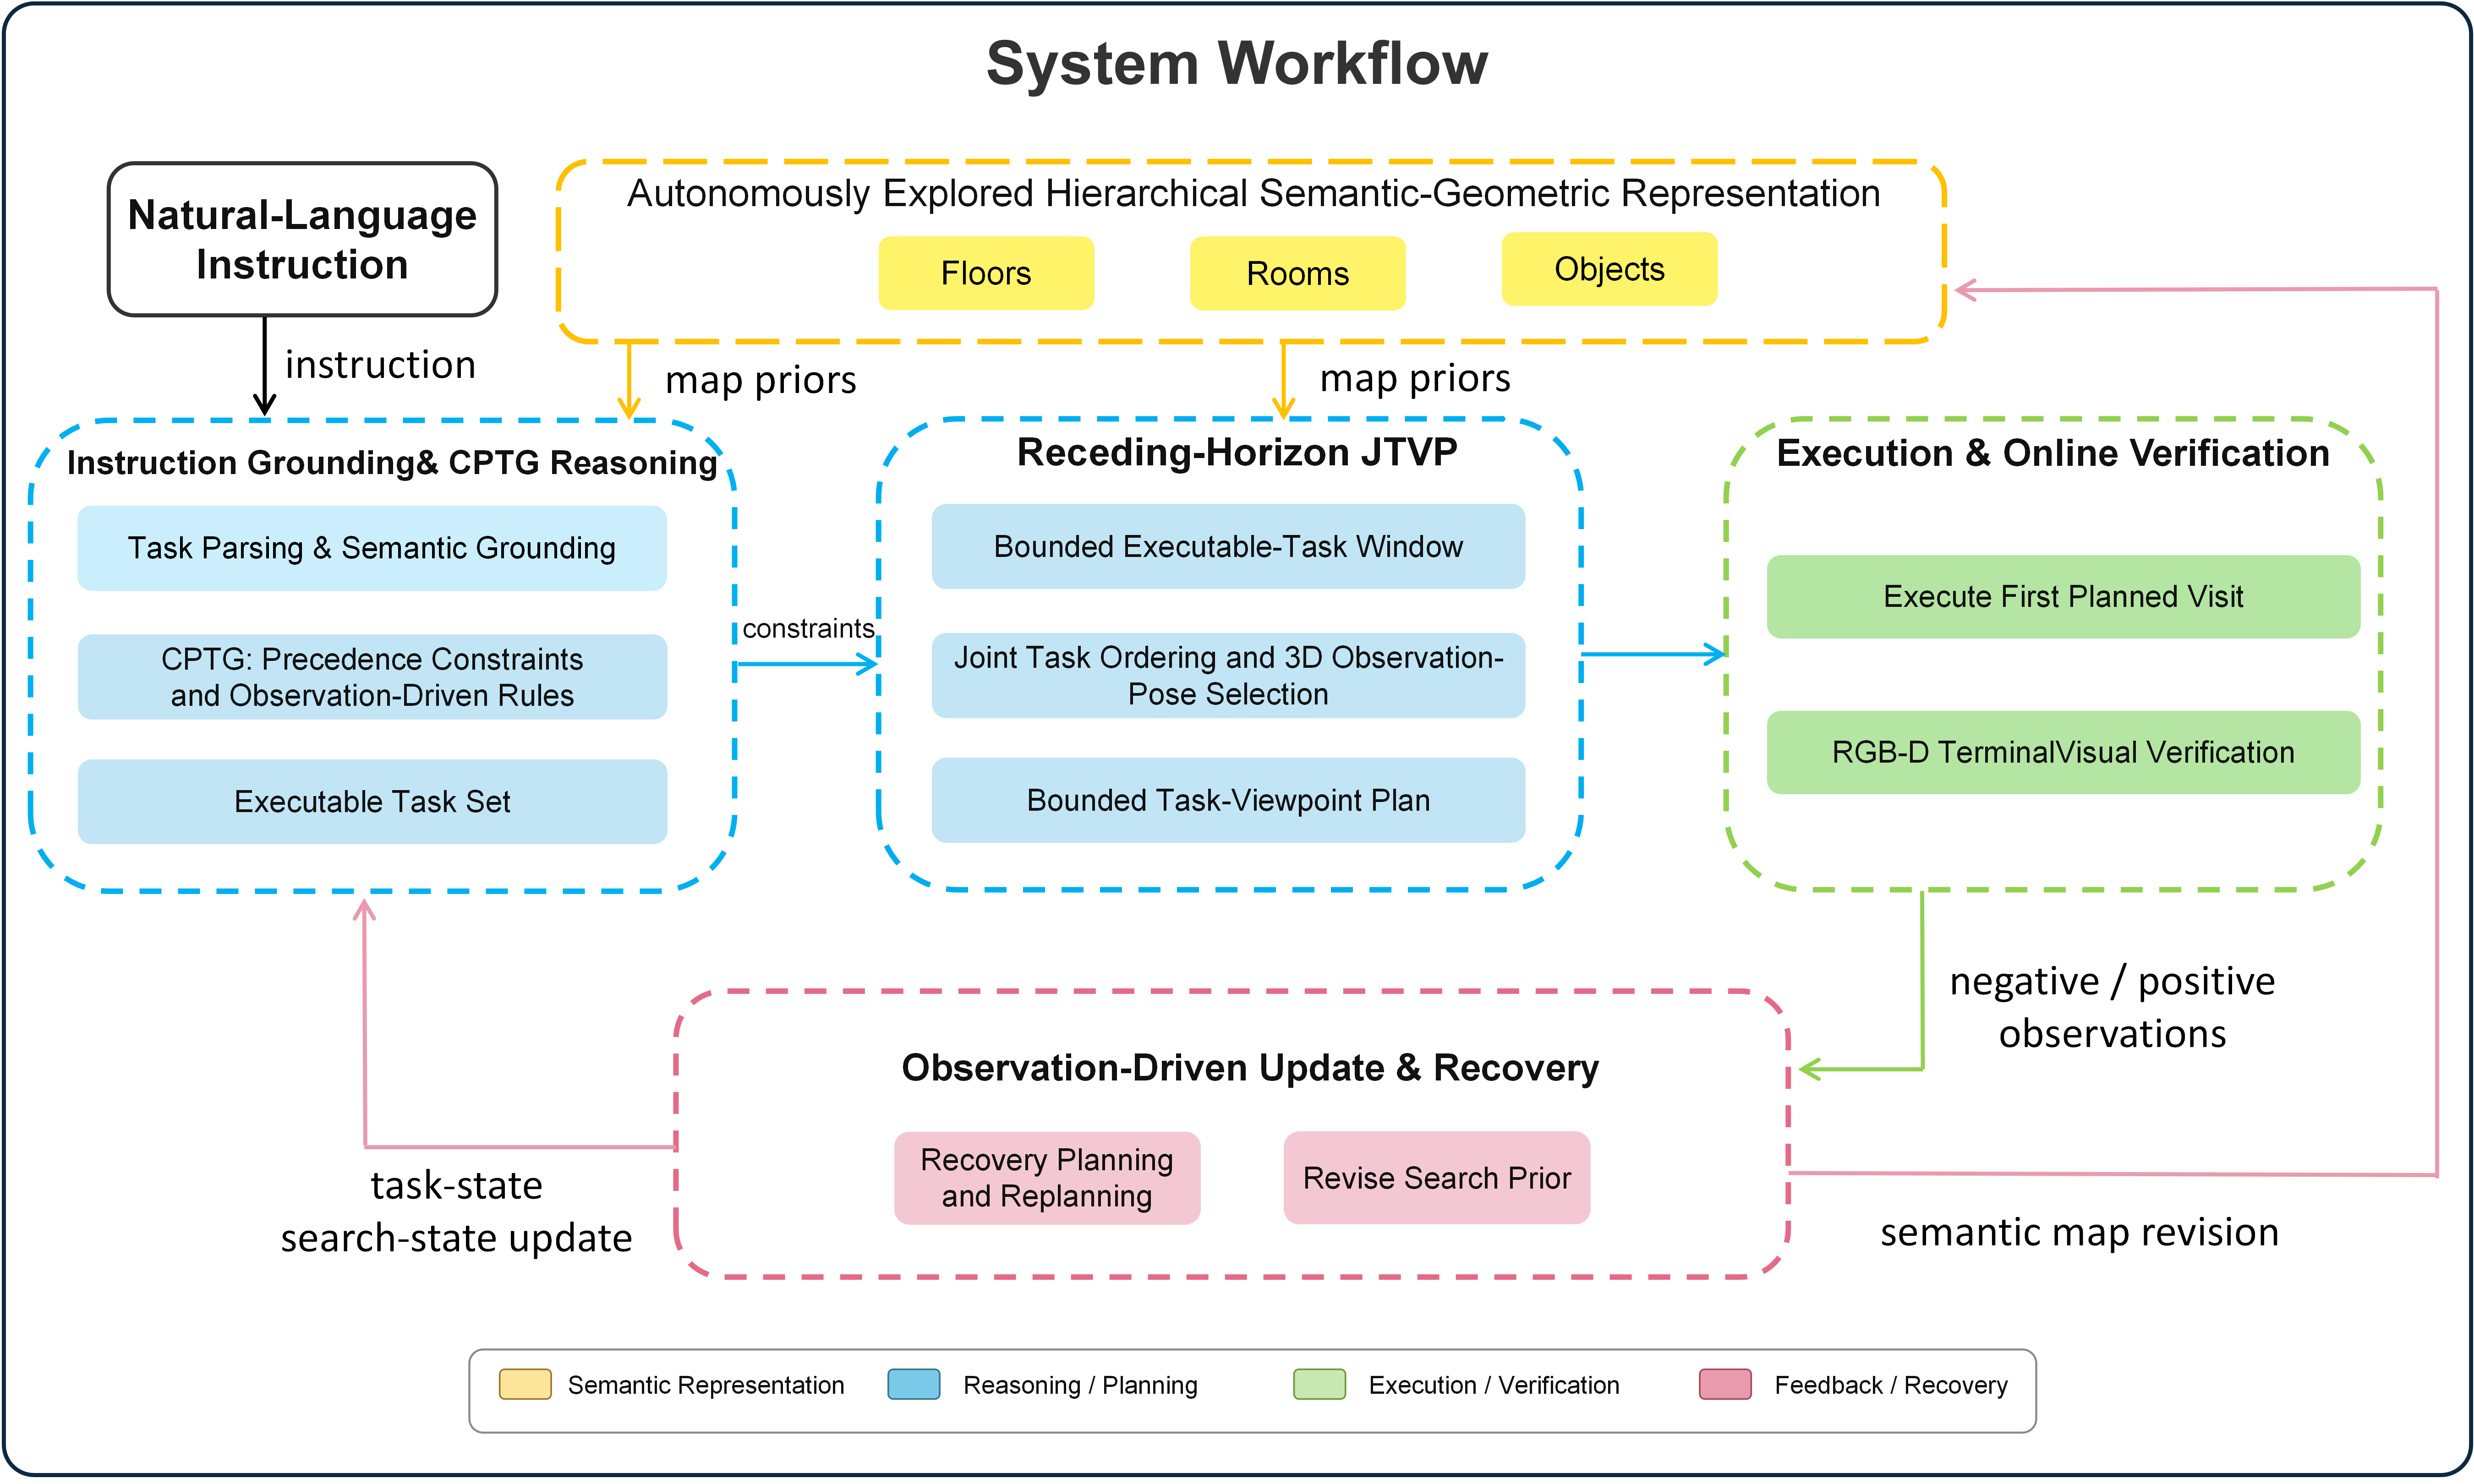
\includegraphics[width=\textwidth]{system_overview.png}
\caption{Overview of LogicFly. A natural-language instruction and an autonomously explored hierarchical semantic--geometric representation are converted into a CPTG and an executable task set. JTVP jointly selects task order and 3D observation poses within a receding horizon. The first planned visit is then executed and verified online; the resulting observations update the task and search states, revise semantic map priors, and trigger recovery and replanning when necessary.}
\label{fig:overview}
\end{figure*}

Several lines of prior work provide important foundations. Iterative VLN studies how previously acquired environmental experience can be reused across repeated navigation episodes~\cite{krantz2023ivln}. VLMaps~\cite{huang2023vlmaps}, ConceptGraphs~\cite{gu2024conceptgraphs}, and HOV-SG~\cite{werby2024hovsg} develop increasingly rich semantic--geometric representations for language-grounded navigation, while long-horizon VLN investigates extended task sequences and persistent memory~\cite{song2024lhvln}. Semantic--geometric planning approaches such as S-Nav~\cite{kremer2023snav}, SayPlan~\cite{rana2023sayplan}, and Optimal Scene Graph Planning (OSGP)~\cite{dai2024osgp} further demonstrate that structured scene semantics can support robot navigation and task planning. However, these directions generally do not jointly address observation-conditioned partial-order task logic, task-specific 3D observation-pose selection, and geometric travel costs within a closed-loop execution framework.

To address these challenges, we develop \textbf{LogicFly}, a language-to-execution framework that couples structured task reasoning, joint task--viewpoint planning, and online visual feedback. We summarize our contributions as follows:
\begin{itemize}
\setlength{\itemsep}{0pt}
\setlength{\parsep}{0pt}
\item \textbf{We propose a Conditional Partial-Order Task Graph (CPTG)} to interpret realistic long-horizon instructions with complex human task logic, explicitly modeling precedence constraints, observation-driven branches, and distinct navigation and verification targets.
\item \textbf{We develop Joint Task--Viewpoint Planning (JTVP)} to jointly optimize task ordering and 3D observation poses within a receding horizon, balancing collision-aware travel cost and observation quality under task constraints.
\item \textbf{We introduce an observation-driven map revision and recovery mechanism} that revises stale semantic priors from negative observations, triggers semantic--geometric replanning, and incrementally incorporates reliable novel objects through multi-view 3D fusion.
\end{itemize}

\section{Related Work}
\subsection{Vision-and-Language Navigation and Spatial Memory}

Vision-and-Language Navigation (VLN) requires embodied agents to follow natural-language instructions from egocentric observations. R2R~\cite{anderson2018r2r}, RxR~\cite{ku2020rxr}, REVERIE~\cite{qi2020reverie}, and VLN-CE~\cite{krantz2020vlnce} established representative settings for instruction following, multilingual navigation, object grounding, and continuous-space navigation, while SOON~\cite{zhu2021soon} emphasizes relational object localization. History-aware methods such as HAMT~\cite{chen2021hamt} and DUET~\cite{chen2022duet} incorporate temporal and graph-structured memory, and Iterative VLN~\cite{krantz2023ivln} studies experience reuse across episodes. Recent work on long-horizon VLN further considers extended task sequences and persistent memory~\cite{song2024lhvln}. PREVALENT~\cite{hao2020prevalent} and ScaleVLN~\cite{wang2023scalevln} improve learned navigation through multimodal pre-training and large-scale instruction--trajectory generation, respectively. In contrast, our focus is execution-time coordination of logically related subtasks.

Spatial memory has progressed from navigation history to explicit semantic--geometric representations. 3D Dynamic Scene Graphs~\cite{rosinol2020dsg} and Hydra~\cite{hughes2022hydra} organize geometry, places, rooms, objects, and agents in structured scene graphs. OpenScene~\cite{peng2023openscene} supports open-vocabulary queries over 3D features, while VLMaps~\cite{huang2023vlmaps}, ConceptGraphs~\cite{gu2024conceptgraphs}, and HOV-SG~\cite{werby2024hovsg} ground language and object semantics in spatial maps and hierarchical scene graphs. A remaining challenge is to turn persistent spatial memory into logic-aware decisions across multiple observation goals. We leverage a hierarchical semantic--geometric representation acquired through autonomous exploration to execute multiple subtasks with partial-order dependencies, conditional branches, and spatial constraints.

\subsection{Scene Graphs and Task--Motion Planning}

Structured scene representations provide a natural bridge between semantic task reasoning and geometric feasibility. SayPlan~\cite{rana2023sayplan} combines 3D scene-graph search, classical planning, and motion-feasibility feedback, while OSGP~\cite{dai2024osgp} converts language instructions into temporal-logic specifications and performs optimal search over hierarchical metric--semantic scene graphs. Related task-and-motion planning methods similarly use hierarchical 3D scene graphs to connect semantic goals with executable motion plans~\cite{ray2024tamp}. Inner Monologue~\cite{huang2023innermonologue} further demonstrates the value of success detection and environment feedback for closed-loop long-horizon planning.

Our formulation explicitly introduces task-conditioned 3D observation poses into the planning state, coupling task ordering, viewpoint selection, and collision-aware travel cost. Unlike general task-and-motion planning, our optimization operates over finite task and observation-pose sets at each receding-horizon planning step.

\subsection{Zero-Shot Vision-and-Language Navigation Agents}

Recent LLM- and VLM-based agents enable navigation without task-specific VLN training. LM-Nav~\cite{shah2023lmnav} composes pretrained language, vision, and navigation models for landmark-level instruction following, while L3MVN~\cite{yu2023l3mvn} uses LLM commonsense to select semantic-map frontiers. NavGPT~\cite{zhou2024navgpt} reasons over visual descriptions, navigation history, and candidate actions, while MapGPT~\cite{chen2024mapgpt} combines mapping with adaptive path planning. SpatialNav~\cite{zhang2026spatialnav} performs global reasoning over spatial scene graphs, whereas VLN-Zero~\cite{bhatt2025vlnzero} integrates rapid exploration, compact scene-graph memory, and neuro-symbolic planning. Open-Nav~\cite{qiao2025opennav} extends zero-shot navigation to continuous environments with open-source language models, and SpatialGPT~\cite{jiang2025spatialgpt} reasons over structured spatial memory.

These methods mainly target navigation toward language-specified goals. Our framework instead executes multiple logically related subtasks within a single instruction, jointly considering partial-order and conditional constraints, spatial relations, task-specific 3D observation poses, and geometric travel costs. The central distinction is therefore the planning abstraction: LogicFly plans over executable task--viewpoint pairs rather than selecting only the next navigation action or goal.

\section{Method}

\textbf{LogicFly} grounds language instructions in a hierarchical semantic--geometric representation. A \textbf{Conditional Partial-Order Task Graph (CPTG)} separates precedence constraints from observation-dependent activation. \textbf{Joint Task--Viewpoint Planning (JTVP)} jointly selects task order and task-conditioned 3D observation poses using collision-aware costs. Online evidence updates task states and search beliefs for recovery and replanning; newly detected instances are fused online and added to the scene graph after execution.

\subsection{Hierarchical Semantic--Geometric Representation}
\label{sec:semantic-representation}

The robot first explores the unknown environment and constructs a reusable hierarchical semantic--geometric representation. Its geometric component $\mathcal M_g$ records occupied, observed-free, and unknown 3D space; its semantic component $\mathcal M_s$ organizes floors, rooms, cross-floor transitions, and open-vocabulary object instances in a shared global frame. FALCON~\cite{zhang2024falcon} supplies exploration trajectories for acquiring RGB-D observations, camera poses, and occupancy evidence. OWLv2~\cite{minderer2023owlv2} provides open-vocabulary 2D detections, Boxer~\cite{detone2026boxer} lifts them into 3D instances, and OccuSG~\cite{cueto2026occusg} organizes rooms. The resulting representation provides semantic entities and regions for task grounding, free space for navigation, and spatial context for viewpoint generation. Figure~\ref{fig:semantic-map-construction} summarizes its construction.

\begin{figure}[t]
\centering
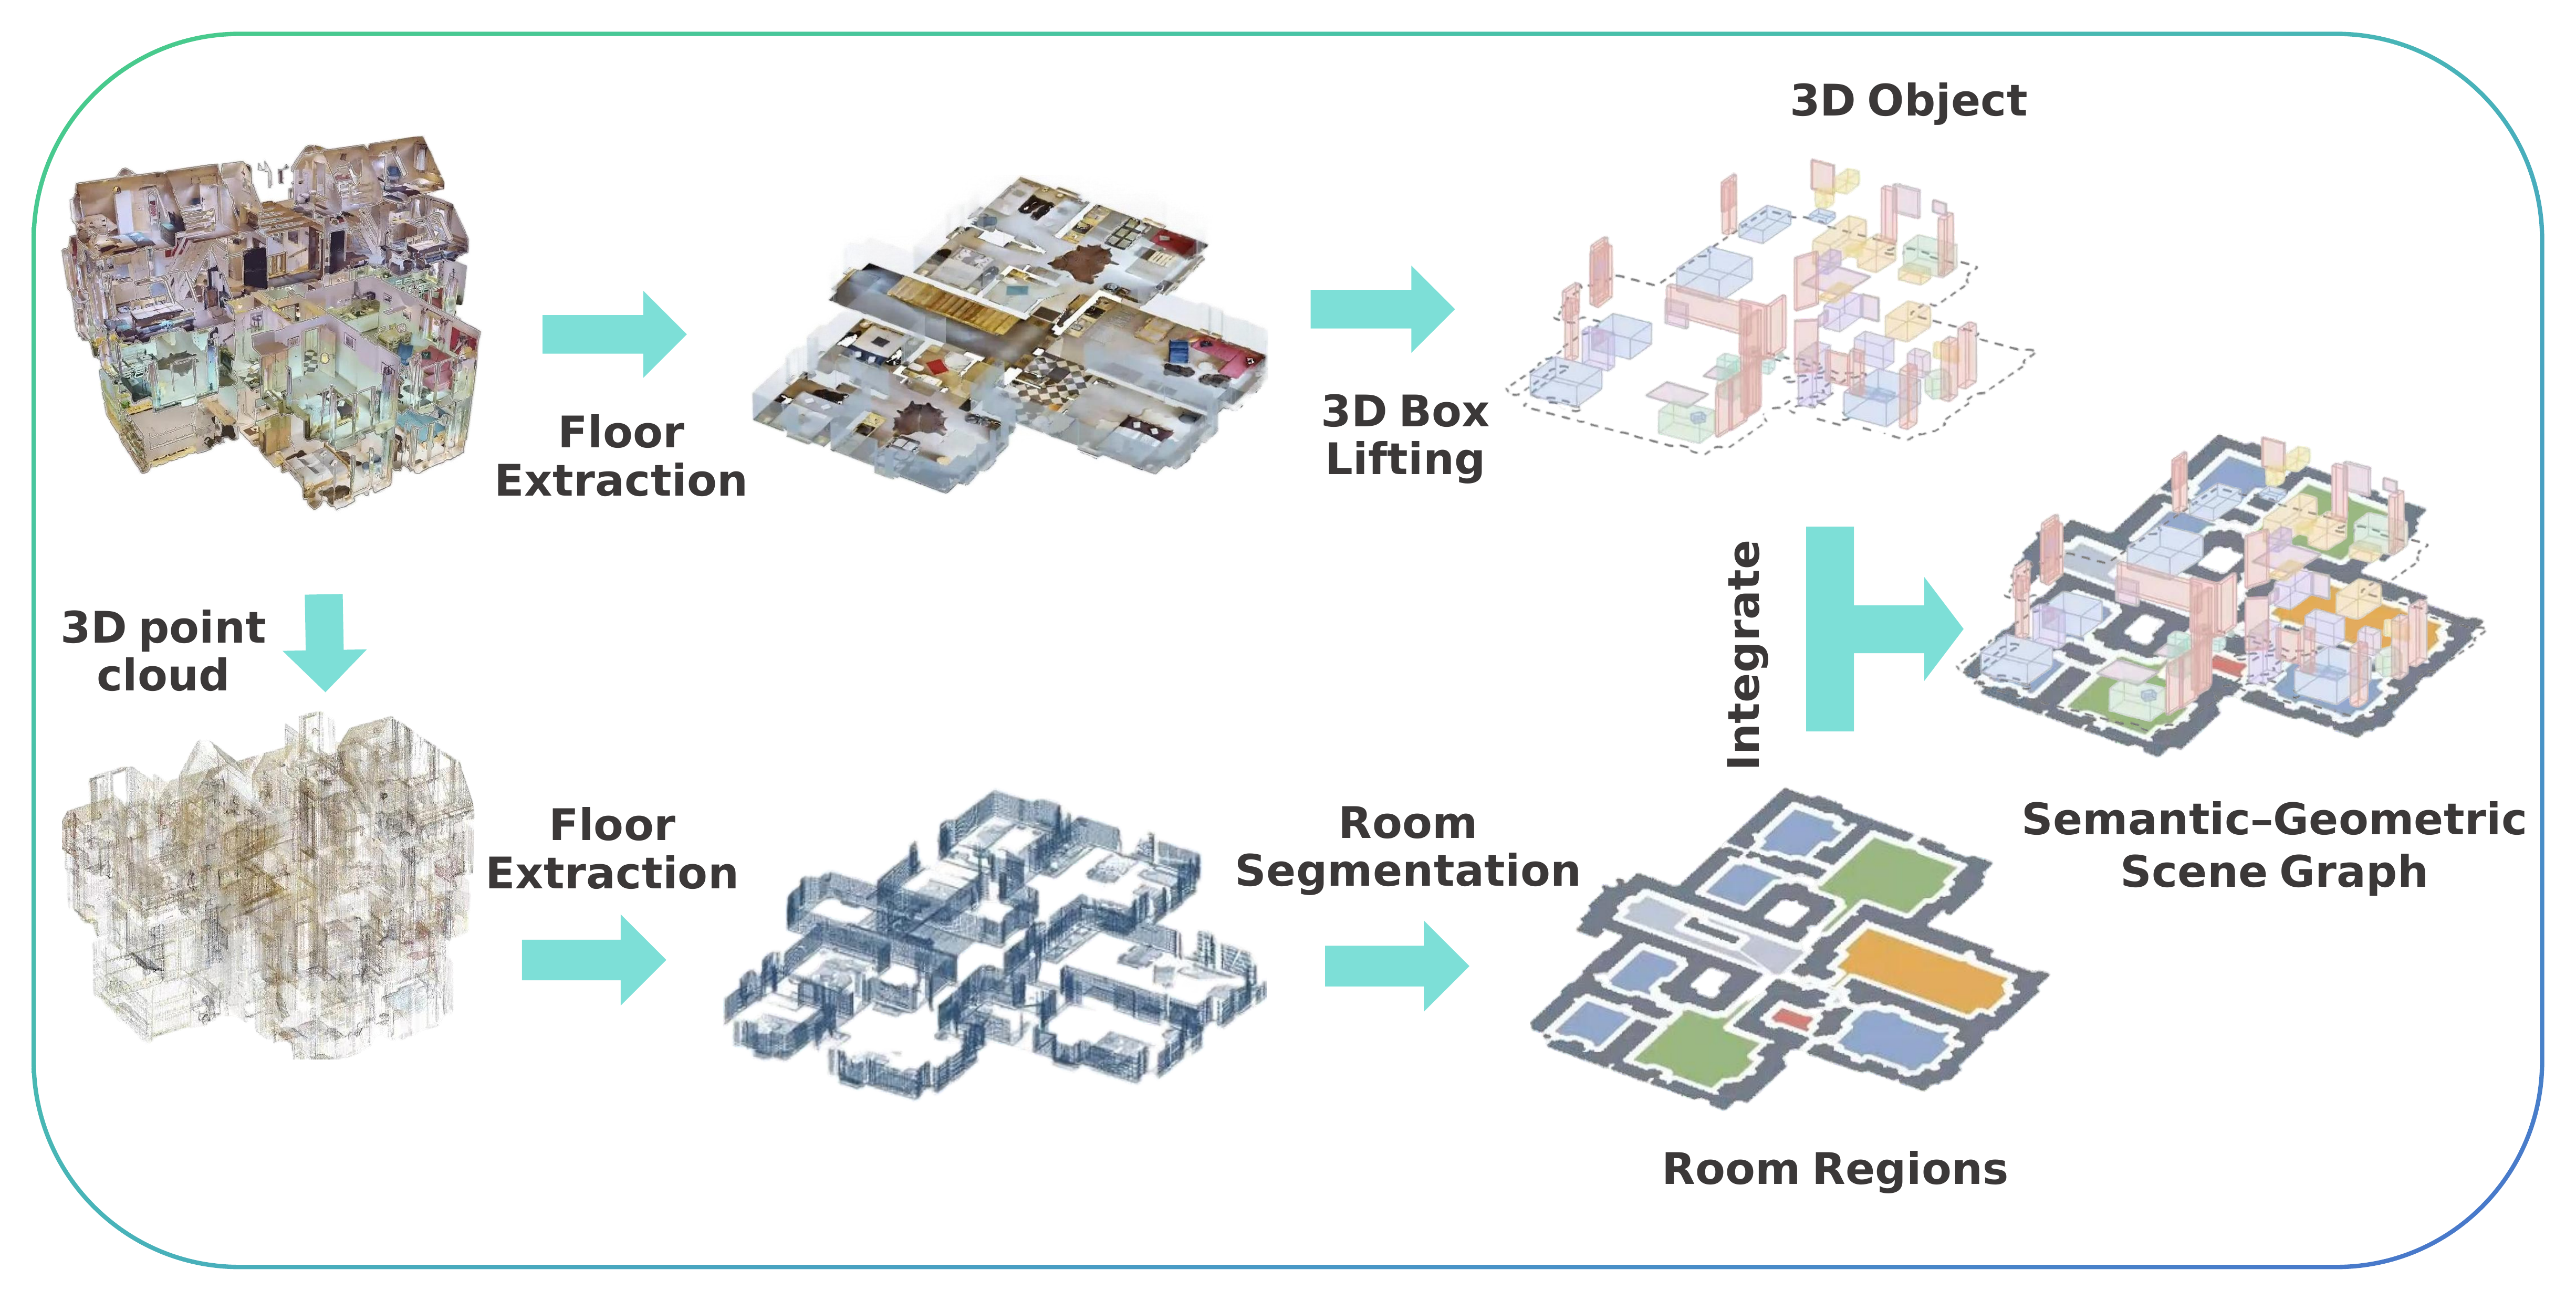
\includegraphics[width=\columnwidth]{autonomous_mapping.png}
\caption{Hierarchical semantic--geometric representation constructed from exploration data by integrating floor/room geometry and 3D object instances.}
\label{fig:semantic-map-construction}
\end{figure}

\subsection{Conditional Partial-Order Task Graph}
\label{sec:cptg}

Given instruction $I$, the parser grounds navigation anchors and room/floor scopes in mapped entities and regions, while specifying semantic targets and verification predicates. These subtasks form a \textbf{Conditional Partial-Order Task Graph}
\begin{equation}
\mathcal G_T=(\mathcal V,\mathcal E_{\mathrm{prec}},\mathcal R_{\mathrm{cond}}),
\end{equation}
where $\mathcal V$ denotes language-grounded subtasks, $\mathcal E_{\mathrm{prec}}$ stores mandatory edges whose transitive closure induces a strict partial order over $\mathcal V$, and $\mathcal R_{\mathrm{cond}}$ contains observation-dependent activation and skip rules. Each task stores its action, semantic target, navigation anchor, verification predicate, spatial constraints, room/floor scope, prerequisites, and search policy. Invalid entity references, inconsistent dependencies, or a cycle in the precedence relation cause rejection before execution. Figure~\ref{fig:cptg} illustrates this representation.

\begin{figure}[t]
\centering
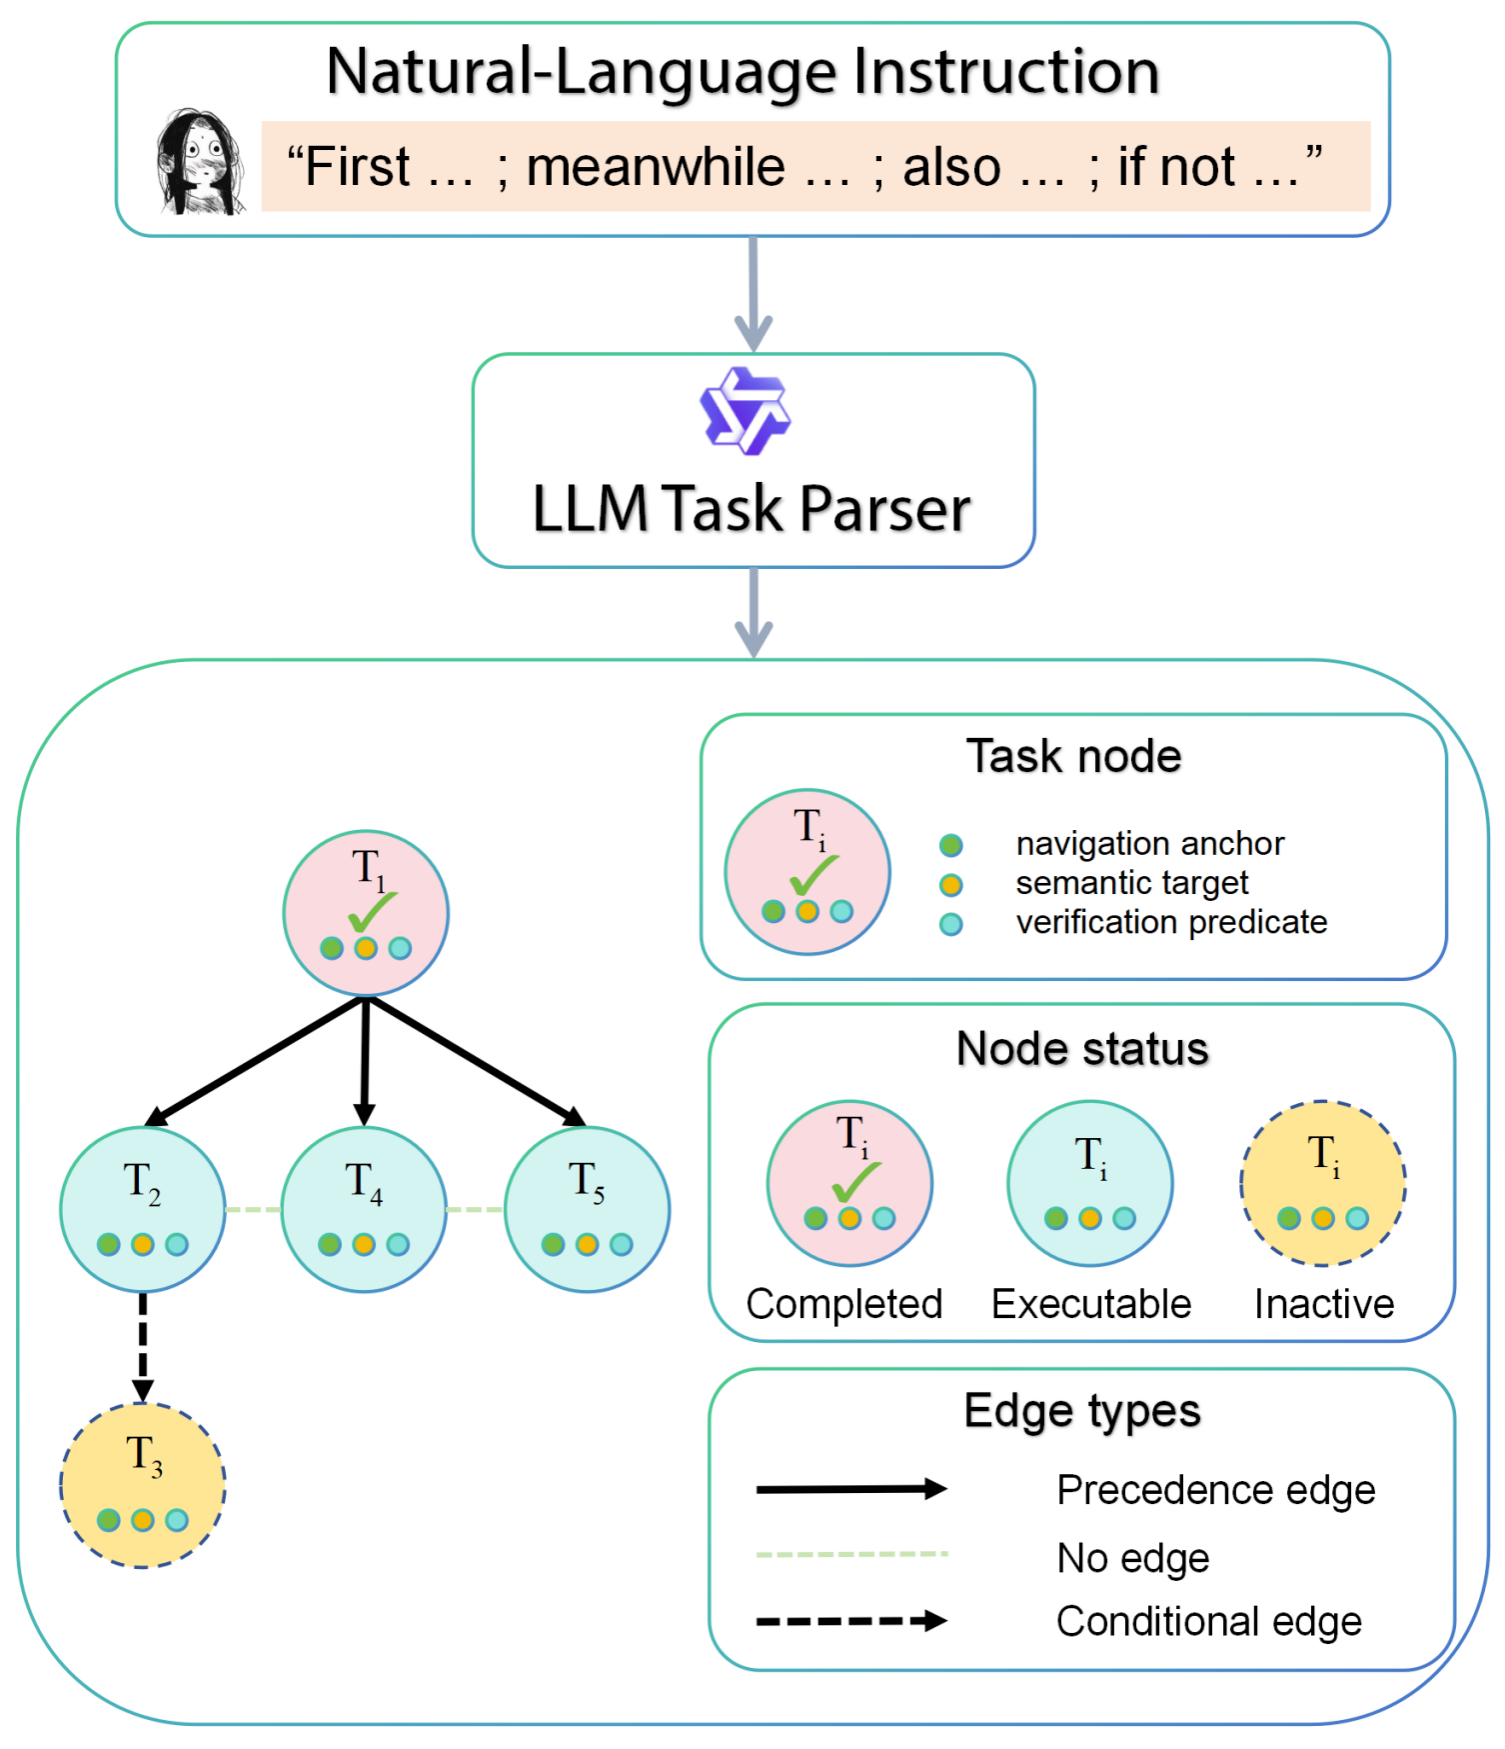
\includegraphics[width=0.92\columnwidth]{conditional_task_graph.png}
\caption{From a natural-language instruction to a CPTG. The task parser constructs task nodes with navigation anchors, semantic targets, and verification predicates; precedence and conditional edges encode mandatory ordering and observation-dependent activation.}
\label{fig:cptg}
\end{figure}

For each task, the \textbf{navigation anchor} defines the observation region, the \textbf{semantic target} specifies the entity to detect, and the \textbf{verification predicate} defines the requested evidence. Spatial relations constrain grounding and candidate generation; their satisfaction is recorded geometrically and required by the strict full-task evaluator.

Let $\mathcal R_t$ contain tasks with resolved outcomes, including negative outcomes, and $\mathcal A_t$ the active pending tasks. With $\operatorname{pred}(i)$ denoting the required predecessors of task $i$, the executable set is
\begin{equation}
\mathcal E_t=
\left\{i\in\mathcal A_t:
\operatorname{pred}(i)\subseteq\mathcal R_t\right\}.
\end{equation}
The rules $\mathcal R_{\mathrm{cond}}$ activate or skip downstream tasks from resolved outcomes. Depending on its observation policy, a conditional source is resolved at the first designated viewpoint or after terminal search. These rules remain separate from mandatory precedence. CPTG supplies executable tasks to JTVP for joint ordering and viewpoint selection.

\subsection{Receding-Horizon Joint Task--Viewpoint Planning}
\label{sec:jtvp}

\textbf{Task-conditioned viewpoints.} For task $i$, its navigation anchor and spatial constraints define a 3D observation region, such as an object, support surface, surrounding area, lower region, or relation-defined area. JTVP generates candidate poses for joint task ordering and viewpoint selection.

The $k$th candidate observation pose is $q_i^k=(x_i^k,y_i^k,z_i^k,\psi_i^k)$, where $(x_i^k,y_i^k,z_i^k)$ is the camera position and $\psi_i^k$ is yaw. Candidates are sampled at multiple distances, azimuths, and feasible heights, with yaw oriented toward the observation region; vertical visibility is handled by candidate height and the camera field of view.

Let $\mathcal P_i$ denote samples from the observation region and $\mathcal V_i(q)\subseteq\mathcal P_i$ the samples visible from $q$ under camera field-of-view and line-of-sight constraints. Geometric coverage is
\begin{equation}
Q_i(q)=\frac{|\mathcal V_i(q)|}{\max(1,|\mathcal P_i|)}.
\end{equation}
Candidates violating occupancy, flight-height, spatial-relation, or required-visibility constraints are discarded. The remaining poses are scored by
\begin{equation}
\begin{aligned}
C_i^{\mathrm{view}}(q)={}&
\beta_d\frac{|d-d_i^{\mathrm{pref}}|}{\ell_0}
+\beta_Q[1-Q_i(q)]\\
&+\beta_z\frac{|z-\bar z_i|}{\ell_0}
+\beta_r\frac{d_i^{\mathrm{ref}}}{\ell_0}
+\beta_b\frac{d_i^{\mathrm{between}}}{\ell_0}.
\end{aligned}
\label{eq:view-cost}
\end{equation}
where $d$ is the sampling distance, $d_i^{\mathrm{pref}}$ is the preferred observation distance, $\bar z_i$ is the mean observation-region height, $d_i^{\mathrm{ref}}$ and $d_i^{\mathrm{between}}$ encode task-dependent spatial relations, and $\ell_0$ is a reference length. Inapplicable terms are zero. Hard feasibility is enforced before scoring so that a low soft cost cannot compensate for an unsafe or unobservable pose. All weights are nonnegative, and their implementation values are reported in Section~IV-A. The retained set $\mathcal Q_i=\{q_i^1,\ldots,q_i^{K_i}\}$ preserves diverse feasible viewpoints.

\textbf{Collision-aware transition costs.} For poses $q_a$ and $q_b$, 3D A$^*$ returns a collision-free polyline $P_t(q_a,q_b)=\{p_1,\ldots,p_N\}$ when reachable. Let $\Delta\psi_{ab}=\operatorname{wrap}(\psi_b-\psi_a)$. Its length and motion-time proxy are
\begin{equation}
\begin{aligned}
L_t(q_a,q_b)&=\sum_{u=1}^{N-1}\|p_{u+1}-p_u\|_2,\\
\widehat T_t(q_a,q_b)&=\max\left\{
\frac{L_t(q_a,q_b)}{v_{xy}},
\frac{|z_b-z_a|}{v_z},
\frac{|\Delta\psi_{ab}|}{\omega_\psi}
\right\}.
\end{aligned}
\label{eq:motion-cost}
\end{equation}
Here, $v_{xy}$ is the nominal translational speed used by the route-length proxy, while $v_z$ and $\omega_\psi$ parameterize vertical and yaw motion.

Figure~\ref{fig:jtvp-illustration} illustrates task-conditioned viewpoint generation and joint selection.

\begin{figure}[t]
\centering
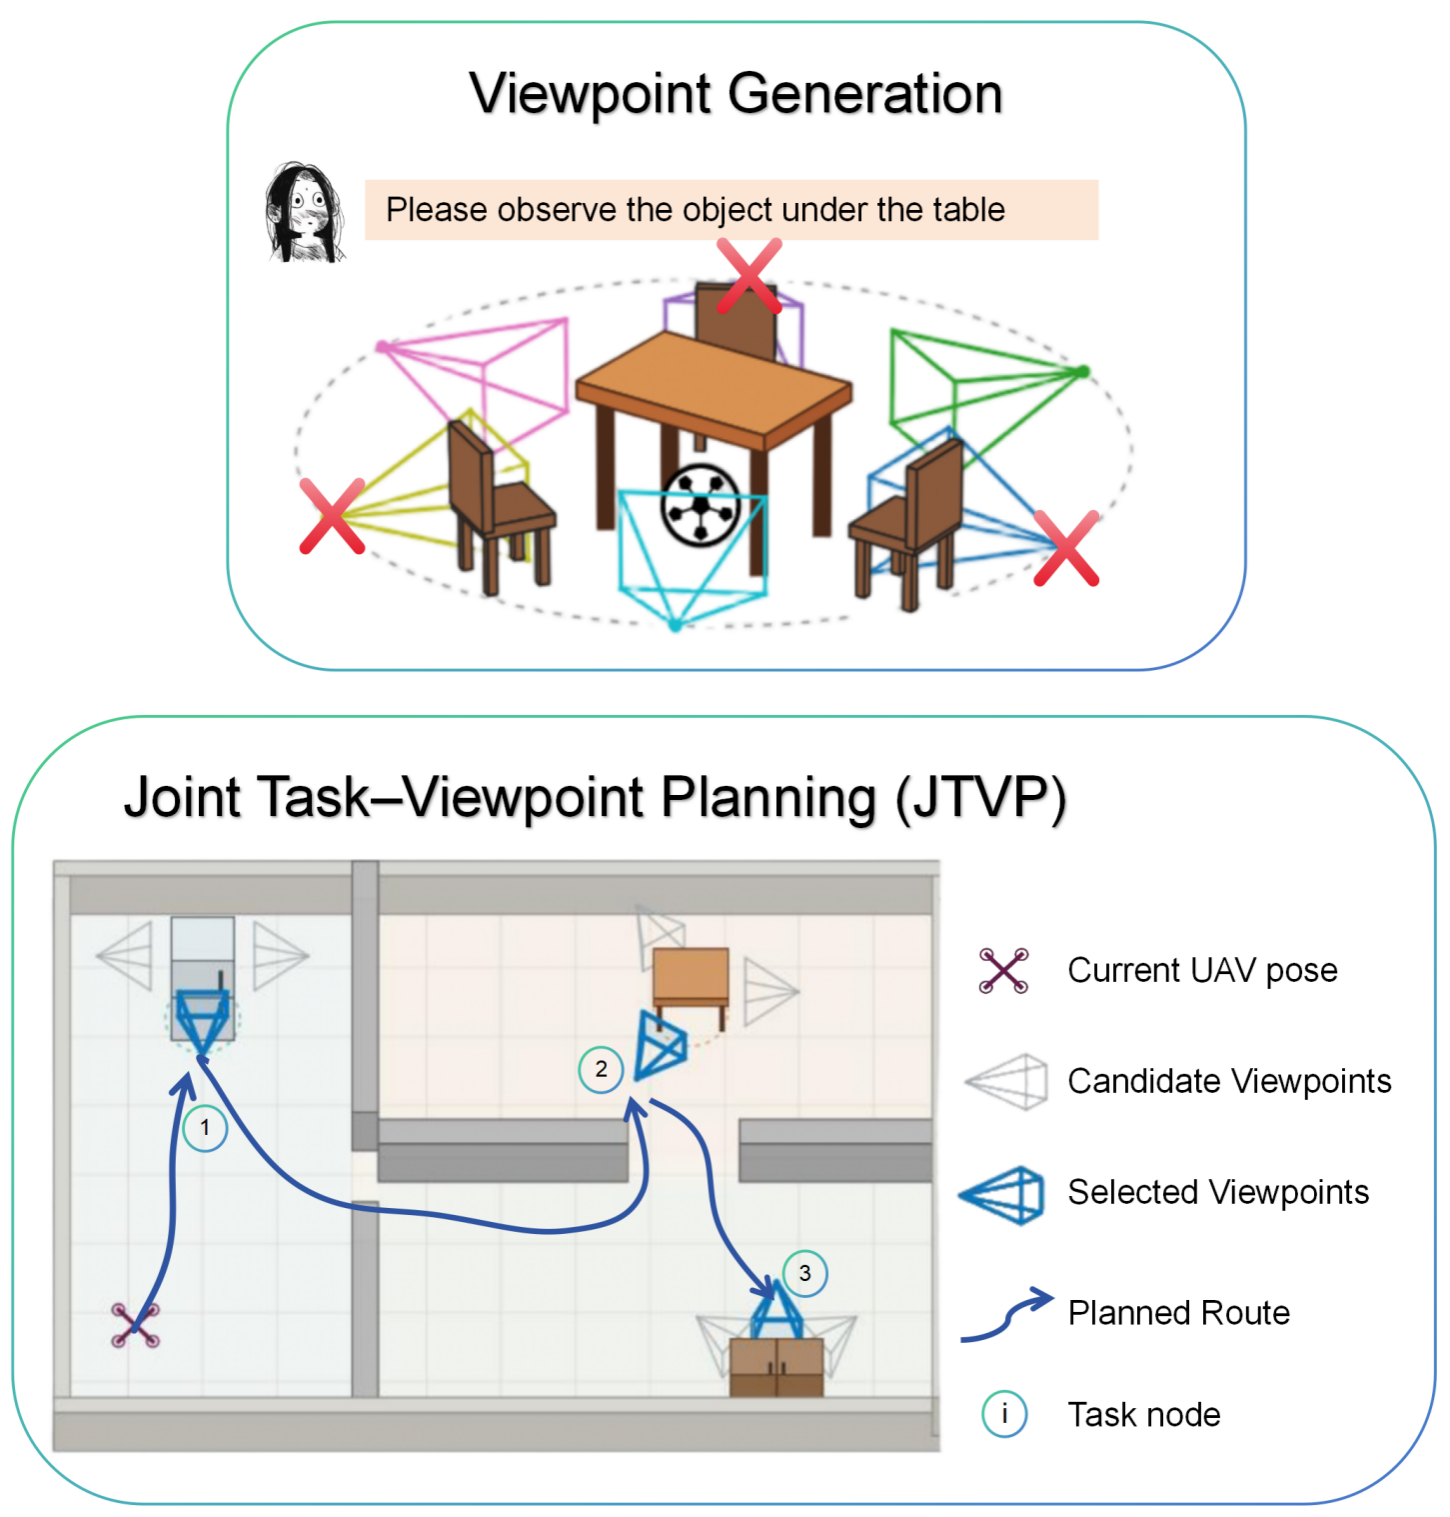
\includegraphics[width=0.88\columnwidth]{joint_task_viewpoint.png}
\caption{Task-conditioned viewpoint generation and joint task--viewpoint planning. Candidate observation poses are generated from semantic and spatial constraints, after which JTVP jointly selects task order, observation poses, and the collision-aware route.}
\label{fig:jtvp-illustration}
\end{figure}

\textbf{Receding-horizon joint optimization.} From CPTG's executable set $\mathcal E_t$, a lightweight estimate using the current robot pose and terminal observation cost selects a window $\mathcal W_t\subseteq\mathcal E_t$, with $|\mathcal W_t|\leq H$ and $H=3$ in the current implementation.

Candidate poses are grouped by physical location and prioritized using current-pose distance, motion-time estimate, and observation score. The retained set $\widetilde{\mathcal Q}_{i,t}\subseteq\mathcal Q_i$ maintains representative viewpoints across semantic locations and is progressively augmented when alternatives are needed.

Given $m=|\mathcal W_t|$, JTVP jointly selects a task ordering $\pi=(\pi_1,\ldots,\pi_m)$ and one observation pose $q_r=q_{\pi_r}^{k_r}$ for each selected task, with $q_0=q_t^{\mathrm{robot}}$. Let $\iota(q)$ denote the task associated with candidate $q$. We use the dimensionless transition score
\begin{equation}
c_t(q_a,q_b)=
\eta_L\frac{L_t(q_a,q_b)}{\ell_0}
+\eta_T\frac{\widehat T_t(q_a,q_b)}{\tau_0}
+\eta_V C_{\iota(q_b)}^{\mathrm{view}}(q_b),
\label{eq:transition-score}
\end{equation}
where $\tau_0$ is a reference time. JTVP solves
\begin{equation}
\begin{aligned}
\min_{\pi,\mathbf k}\quad
&\sum_{r=1}^{m}c_t(q_{r-1},q_r)\\
\mathrm{s.t.}\quad
&q_r\in\widetilde{\mathcal Q}_{\pi_r,t},\qquad
L_t(q_{r-1},q_r)<+\infty .
\end{aligned}
\label{eq:jtvp}
\end{equation}
The joint planning problem is solved using subset dynamic programming. Let $D(S,i,k)$ be the minimum accumulated cost of visiting task subset $S\subseteq\mathcal W_t$ and ending at candidate $k$ of task $i$. The initialization, recurrence, and final cost are
\begin{equation}
\begin{aligned}
D(\{i\},i,k)&=c_t(q_0,q_i^k),\\
D(S\cup\{j\},j,\ell)&=
\min_{i\in S,k}\left[D(S,i,k)+c_t(q_i^k,q_j^\ell)\right],\\
J_t^\star&=\min_{i\in\mathcal W_t,\;k}D(\mathcal W_t,i,k).
\end{aligned}
\label{eq:subset-dp}
\end{equation}
Backtracking returns the task order and observation poses. Only the first visit is executed before replanning from the updated robot pose, task state, candidate set, and semantic evidence, preserving multi-task lookahead while adapting later visits to new observations.

\subsection{Closed-Loop Execution with Observation-Driven Semantic Map Updates and Replanning}
\label{sec:recovery}

After JTVP selects the next task and observation pose, the corresponding A$^*$ route is converted into a collision-checked cubic B-spline trajectory. RGB observations acquired during motion contribute semantic evidence, while terminal RGB-D observations provide open-vocabulary detections, depth-based 3D projections, and geometric verification cues. A positive online verification advances the task state. A negative terminal observation is handled according to the task-specific not-found policy: it may trigger another local viewpoint, bounded semantic recovery, a terminal absence result, or an observation-dependent branch.

Detections are lifted into the global frame using depth and camera pose. Spatial consistency associates same-category observations with mapped instances; unmatched detections accumulate across views for scene-graph revision.

For tasks configured for semantic recovery, LogicFly distinguishes three levels of negative evidence. A \textbf{pose-level miss} removes the attempted candidate while keeping the task active. \textbf{Region-level exhaustion} invokes alternative room--functional-region hypotheses grounded in the hierarchy; these hypotheses become geometric observation regions and are ranked using semantic relevance, coverage, and travel cost. A \textbf{task-level negative outcome} is produced when the task-specific stopping condition is reached, after which CPTG updates downstream logic. Within semantic recovery, newly covered portions of an unproductive region reduce its belief, shifting search toward alternative hypotheses.

Novel detections are accumulated online through spatially consistent multi-view fusion and materialized in the updated scene graph after execution. Thus, task states and semantic-region beliefs can affect replanning within the current execution, whereas newly created object instances support later use of the revised map.

After each terminal verification, the system updates the task state, candidate poses, and semantic search prior, recomputes $\mathcal E_t$, and invokes JTVP from the current robot pose. When a task reaches a task-level outcome, CPTG additionally updates $\mathcal R_t$ and evaluates $\mathcal R_{\mathrm{cond}}$ to activate or skip downstream conditional tasks. This closes the loop among task logic, 3D observation, geometric motion, and online semantic evidence.

\begin{table*}[t!]
\caption{Comparison with state-of-the-art methods on the six-scene HM3D benchmark. Each method is evaluated on 180 single-target and 180 multi-target episodes. Bold denotes the best result.}
\label{tab:main}\centering\small\setlength{\tabcolsep}{4pt}
\begin{tabular}{lrrrrrrrrrr}\toprule
&\multicolumn{5}{c}{Single-target}&\multicolumn{5}{c}{Multi-target full task}\\
\cmidrule(lr){2-6}\cmidrule(lr){7-11}
Method&TL$\downarrow$ (m)&SR$\uparrow$ (\%)&NE$\downarrow$ (m)&SPL$\uparrow$&CT$\downarrow$ (s)&TL$\downarrow$ (m)&SR$\uparrow$ (\%)&NE$\downarrow$ (m)&SPL$\uparrow$&CT$\downarrow$ (s)\\\midrule
SpatialNav&9.399&18.33&9.009&0.174&25.881&\NA&0.00&\NA&\NA&\NA\\
VLN-Zero&4.684&19.44&9.055&0.153&138.532&\NA&0.00&\NA&\NA&\NA\\
SpatialGPT&8.866&31.67&8.565&0.235&112.851&\NA&0.00&\NA&\NA&\NA\\
MapGPT&11.500&37.22&6.853&0.271&43.040&\NA&0.00&\NA&\NA&\NA\\
OSGP&8.285&41.11&1.342&0.874&159.751&8.559&0.00&2.725&0.000&\NA\\
LogicFly&8.750&\textbf{93.33}&1.541&0.867&\textbf{8.246}&24.734&\textbf{71.11}&\textbf{1.185}&\textbf{0.718}&\textbf{12.101}\\\bottomrule
\end{tabular}
\end{table*}

\section{Experiments}
We evaluate LogicFly through simulation, real-world UAV experiments, and ablation studies, covering benchmark performance, practical deployment, and the contributions of CPTG and JTVP.

\subsection{Experimental Setup}
\textbf{Evaluation benchmark.}
We evaluate all methods on six HM3D~\cite{ramakrishnan2021hm3d} scenes: 00070, 00166, 00273, 00290, 00337, and 00409. Each scene contains five single-target short-instruction tasks and five multi-target long-instruction tasks covering single- and cross-floor navigation, ordering constraints, conditional execution, semantic recovery, and verified absence. Each task is tested from three fixed starting positions with two repetitions, resulting in 180 episodes per task family and method.

\textbf{Evaluation metrics.}
We report Trajectory Length (TL), Navigation Error (NE), task Success Rate (SR), Success weighted by Path Length (SPL), and Completion Time (CT). TL denotes mean executed trajectory length. Success is defined strictly at the full-task level: every required subtask outcome and realized logical, spatial, disambiguation, and recovery constraint must be satisfied, while skipped conditional branches must not be visited. SPL is computed as
\begin{equation}
\mathrm{SPL}_e=S_e\frac{L_e^{\mathrm{ref}}}
{\max(L_e^{\mathrm{ref}},L_e)},
\end{equation}
where $S_e$ is strict binary full-task success, $L_e$ is the executed trajectory length, and $L_e^{\mathrm{ref}}$ is the branch- and order-consistent reference route. CT is reported over successful episodes; NE and SPL are N/A for verified-absence tasks without a target position.

\textbf{Implementation details.}
Our runner executes precompiled CPTGs and uses local OWLv2 for online verification, while semantic recovery can invoke Qwen3.8-Flash\footnote{Alibaba Cloud Model Studio, model ID \texttt{qwen3.8-flash}: \url{https://help.aliyun.com/en/model-studio/qwen3-8-flash} (accessed Sep. 15, 2026).} with temperature 0 and thinking disabled. All planning parameters are fixed across scenes and tasks: $(v_{xy},v_z,\omega_\psi)=(1.0~\mathrm{m/s},0.5~\mathrm{m/s},1.0~\mathrm{rad/s})$, $(\ell_0,\tau_0)=(1~\mathrm{m},1~\mathrm{s})$, $(\beta_d,\beta_Q,\beta_z,\beta_r,\beta_b)=(1,1,0.10,0.15,0.15)$, and $(\eta_L,\eta_T,\eta_V)=(1,0.25,2)$. CT excludes preparation and post-hoc evaluation, and each process has a 240 s wall-clock limit. All methods use identical cases, starts, and repetitions; unsupported cases, timeouts, and infrastructure failures are counted as failures.

\subsection{Comparison with State-of-the-Art Methods in Simulation}
We compare LogicFly with HM3D adaptations of MapGPT~\cite{chen2024mapgpt}, OSGP~\cite{dai2024osgp}, SpatialGPT~\cite{jiang2025spatialgpt}, SpatialNav~\cite{zhang2026spatialnav}, and VLN-Zero~\cite{bhatt2025vlnzero}. As shown in Table~\ref{tab:main}, LogicFly achieves a 93.33\% SR on single-target tasks, outperforming the strongest baseline by 52.22 percentage points, while attaining the lowest CT of 8.246 s and an SPL of 0.867.

On multi-target long-instruction tasks, LogicFly achieves a 71.11\% full-task SR, with an NE of 1.185 m and an SPL of 0.718 where geometric reference routes are defined. These results demonstrate its ability to coordinate multiple targets, logical dependencies, conditional outcomes, and online recovery within a unified execution loop.

Figure~\ref{fig:simulation-execution} presents a qualitative execution example in a three-floor Habitat environment. LogicFly completes the cross-floor route and all required subtasks, with terminal views providing visual evidence for each successful outcome.

\begin{figure}[t]
\centering
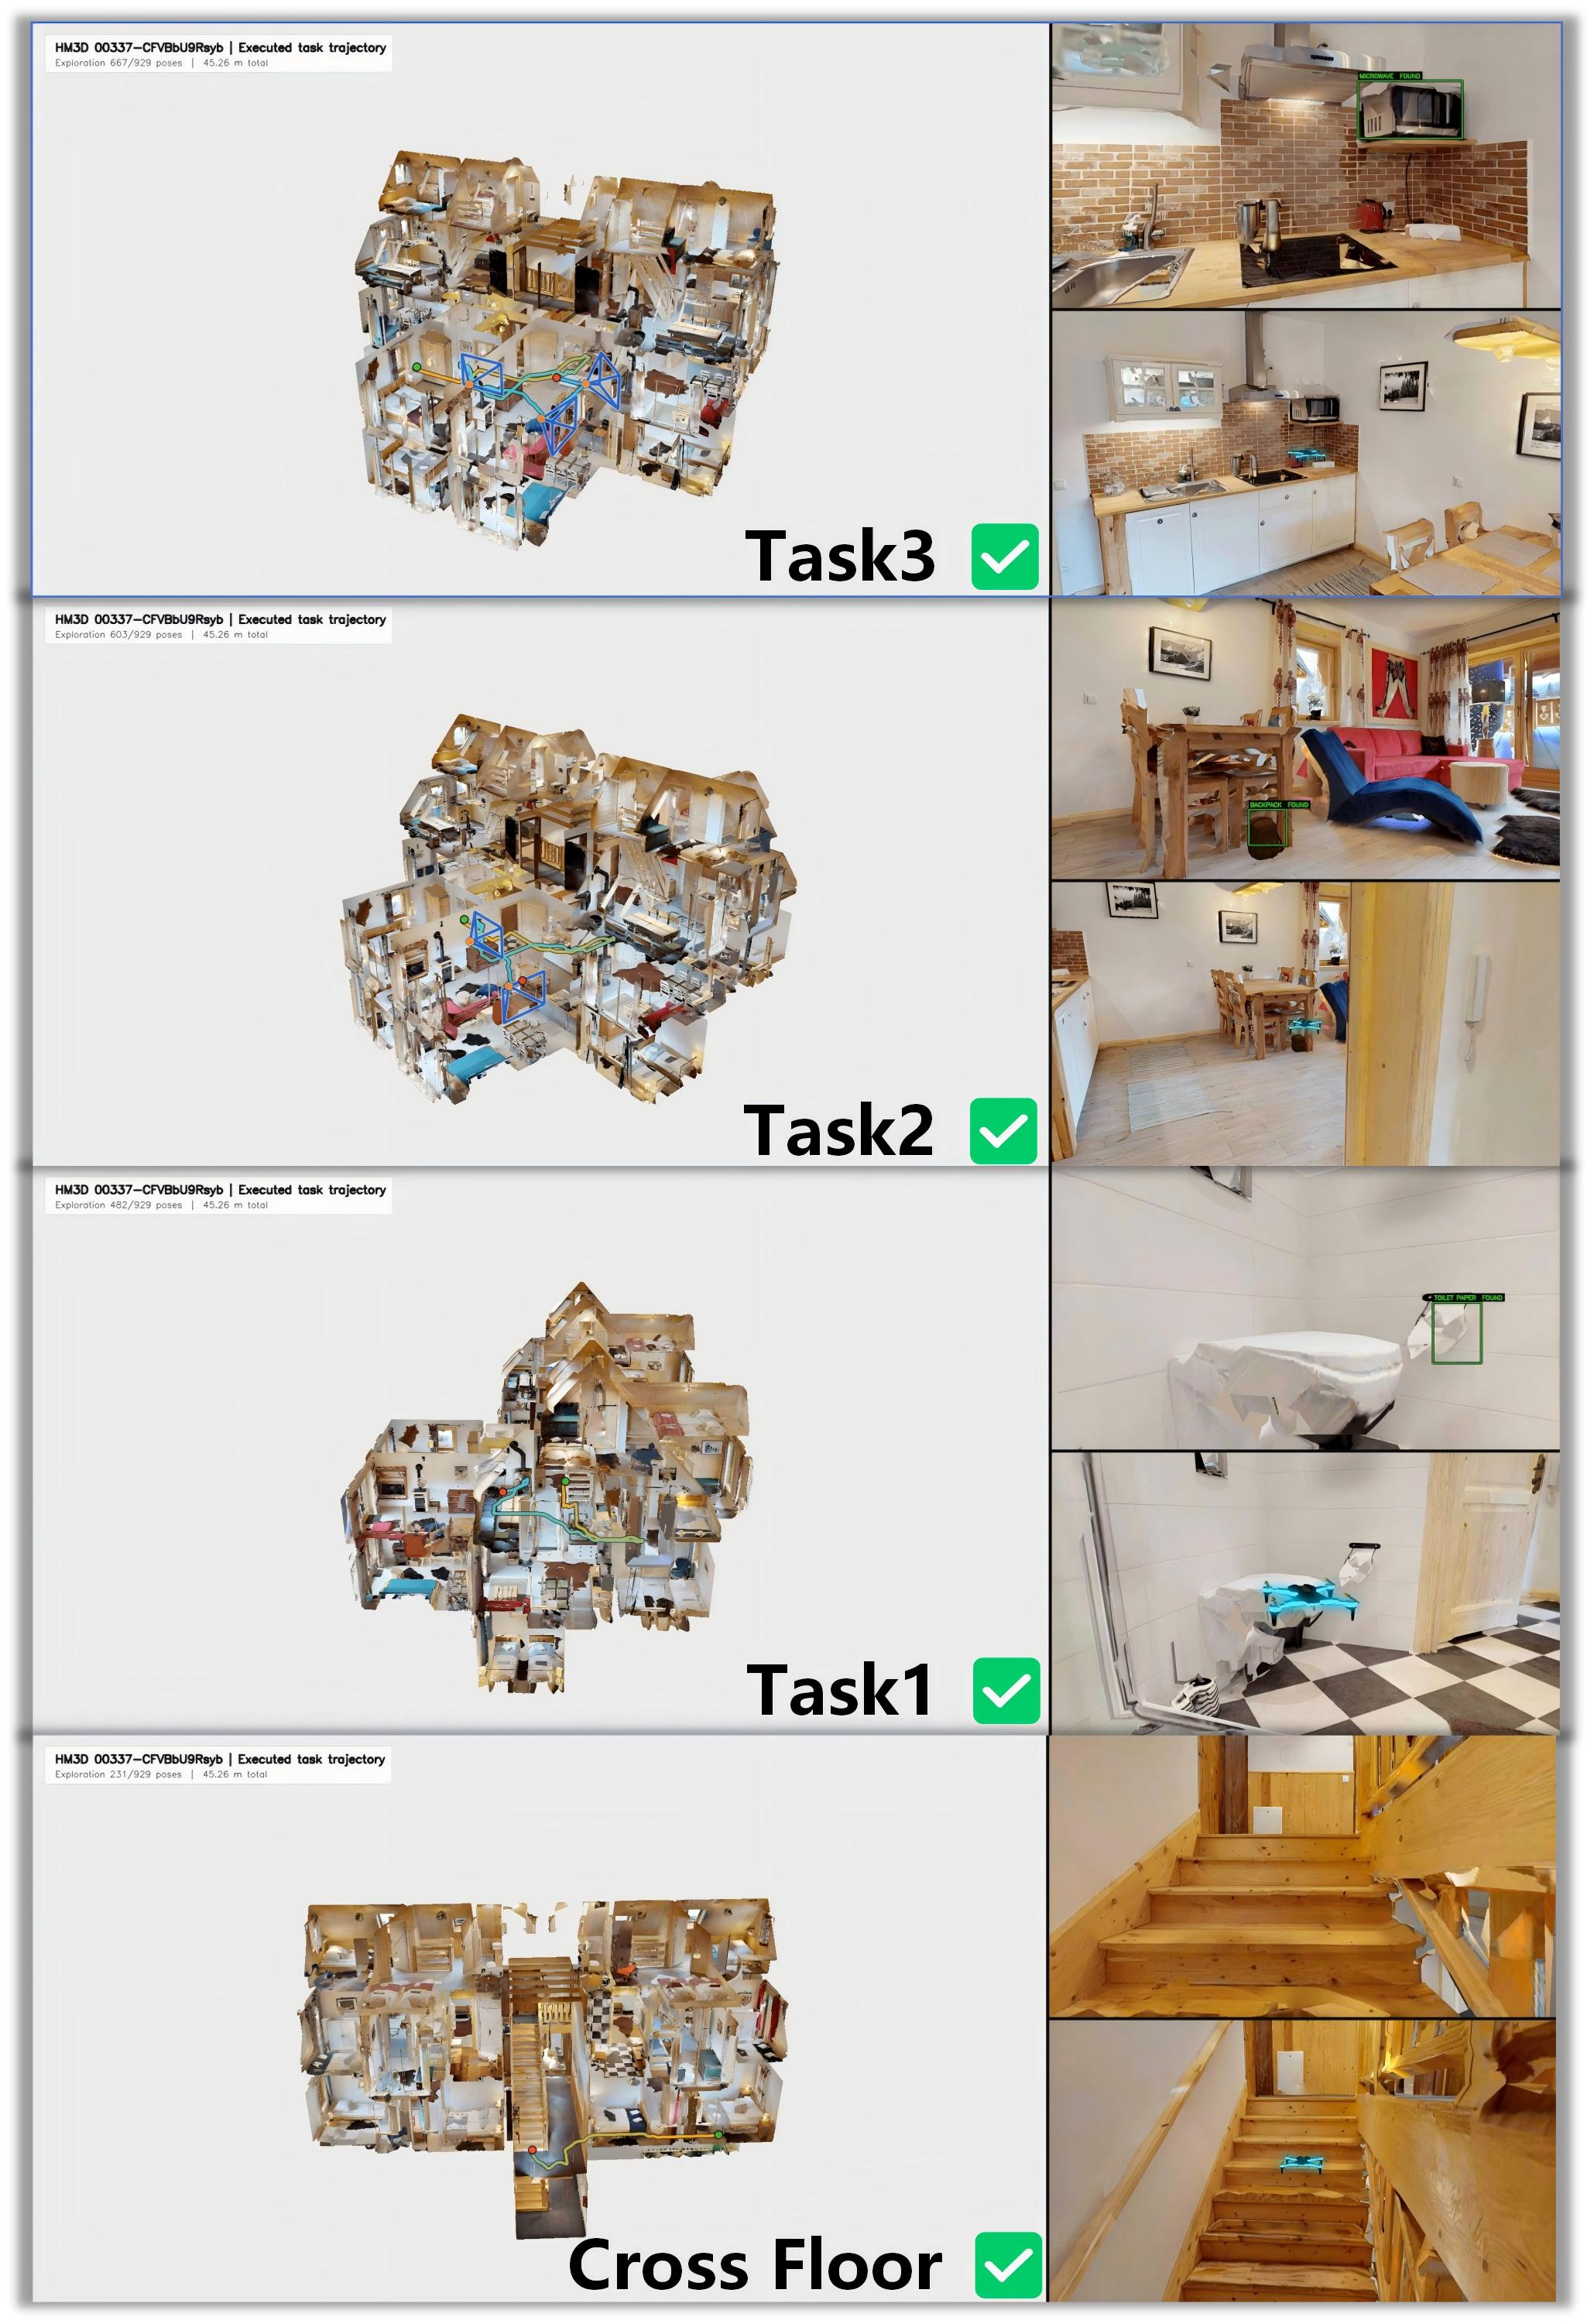
\includegraphics[width=0.82\columnwidth]{simulation_execution.jpg}
\caption{Successful execution of a complex multi-target task in a three-floor Habitat environment. The panels include successful target recognition from the UAV's first-person view, third-person views of the UAV during execution, and the complete 3D trajectory. All required subtasks are successfully completed.}
\label{fig:simulation-execution}
\end{figure}

All baselines retain their native planning, action, and stopping interfaces. MapGPT, SpatialGPT, SpatialNav, and VLN-Zero do not expose the structured multi-target outputs required by the full-task evaluator, while the available OSGP runtime lacks online visual verification for conditional and recovery decisions.

\subsection{Evaluation in Real-World Environments}
\textbf{Experimental platform.}
We conduct real-world experiments using a custom-built quadrotor equipped with an NVIDIA Jetson Orin NX (16 GB), a PX4 flight controller, a Livox Mid-360 LiDAR, and an Intel RealSense D435 depth camera. The D435 provides synchronized $640\times480$ RGB and depth observations for online verification and 3D projection. FAST-LIO~\cite{xu2021fastlio} provides onboard localization, while LiDAR-based occupancy mapping supports real-time trajectory optimization. The UAV is constrained to a maximum linear velocity of $1.0~\mathrm{m/s}$, linear acceleration of $1.0~\mathrm{m/s^2}$, and angular velocity of $1.0~\mathrm{rad/s}$.

As illustrated in Fig.~\ref{fig:real-world-main}, LogicFly completes a three-target instruction end to end with a physical UAV in a real multi-room environment. The 3D reconstruction provides only a bird's-eye visualization of the physical layout and executed trajectory; all navigation, observation, and verification are performed in the real environment.

\subsection{Ablation Studies}
We evaluate CPTG and JTVP on 30 multi-target long-instruction cases spanning six HM3D scenes: 5 ordered, 5 freely schedulable (parallel), 5 conditional-branch, 6 verified-absence, 7 semantic-recovery/additional-exploration, 1 spatial-relation, and 1 target-disambiguation case. Single-target cases are excluded because they do not exercise multi-task scheduling. Each case is run twice from one fixed starting position, yielding 60 episodes per variant.

All variants are executed end to end using the native Habitat runner, online OWLv2 verification, and the same strict evaluator. They share identical scene representations, start poses, motion constraints, termination rules, and evaluation settings. \emph{w/o CPTG} removes task dependencies, conditional rules, and task-conditioned candidate generation, retaining only target labels, coarse room/floor scopes, generic observation constraints, and fixed language order. \emph{CPTG + fixed views} retains CPTG and task-order optimization but uses one independently selected fixed observation pose per task. \emph{CPTG + JTVP} jointly optimizes task ordering and observation viewpoints. The evaluator requires every required outcome and effective order, forbids visits to skipped branches, and checks spatial/reference constraints.

\begin{table}[t]
\caption{End-to-end ablation on 30 multi-target tasks with 60 episodes per variant.}
\label{tab:ablation}\centering\footnotesize\setlength{\tabcolsep}{4pt}
\begin{tabular}{lrrr}\toprule
Variant&SR$\uparrow$ (\%)&SPL$\uparrow$ (\%)&TL$\downarrow$ (m)\\\midrule
w/o CPTG&60.0&43.9&24.89\\
CPTG + fixed views&73.3&55.1&27.47\\
CPTG + JTVP&73.3&69.0&21.02\\\bottomrule
\end{tabular}
\end{table}

As shown in Table~\ref{tab:ablation}, \emph{CPTG + JTVP} achieves a 73.3\% SR and improves SPL from 55.1\% with \emph{CPTG + fixed views} to 69.0\%, while reducing mean trajectory length from 27.47 m to 21.02 m. This indicates that joint task--viewpoint planning primarily improves route efficiency. The \emph{w/o CPTG} variant reduces SR to 60.0\% and introduces failures such as skipped-branch visits and violations of spatial/reference constraints. Three infrastructure failures in \emph{CPTG + JTVP} are counted as failures.

\section{Conclusion}
We presented \textbf{LogicFly}, a language-guided aerial navigation framework built around CPTG and JTVP. CPTG separates precedence and observation-triggered branches; JTVP selects task order and observation poses with 3D path and terminal costs within a bounded window. Verification and constrained recovery update subsequent decisions.

Under a strict full-task evaluation, our method achieves strong performance on multi-target tasks with complex logic. Ablation studies further verify the role of CPTG in executing complex task logic and the contribution of JTVP to path efficiency and viewpoint planning. In addition, we deploy the system on a custom quadrotor UAV and complete multi-target tasks with logical dependencies in real indoor rooms, demonstrating its practical deployability. We hope this work will encourage the development of vision-and-language navigation beyond single-goal route following toward efficient closed-loop autonomous execution of tasks with complex logic.
\bibliographystyle{IEEEtran}
\bibliography{references}
\end{document}
